% !TeX program = xelatex
%==============================================================
%  Python金融数据分析 · 第5章 Matplotlib可视化
%  绘图方法参考教材第7章；统一案例为 UCI Bike Sharing 日表
%  授课对象：本科金融系学生（已学完第2-4章）
%  编译：xelatex chapter5.tex（编译两遍）
%==============================================================
\documentclass[9pt]{ctexbeamer}

%%%%-----导入宏包-----%%%%
\usepackage{style/shubeamer}   % SHU 主题（配色、帧标题、页脚、Python代码样式）
\usepackage{amsmath,amsfonts,amssymb,bm}
\usepackage{graphicx,hyperref,url}
\usepackage{subcaption}
\usepackage{booktabs}
\usepackage[super,square]{natbib}
\usepackage{wrapfig}          % 文字绕排
\usepackage{calligra}         % 结尾页花体字

%%%%-----设置字体-----%%%%
\setmainfont{CMU Serif}
\setsansfont{CMU Sans Serif}

%%%%-----常用自定义颜色（正文可直接使用）-----%%%%
\definecolor{nvidia}{RGB}{102,156,28}
\definecolor{red}{RGB}{184,13,73}
\definecolor{orange}{RGB}{242,151,36}
\definecolor{darkteal}{RGB}{43,106,108}
\definecolor{darkblue}{RGB}{4,37,58}

%%%%-----每节开始时自动显示当前节目录-----%%%%
\AtBeginSection[]
{
	\begin{frame}<beamer>
		\frametitle{\textbf{目录}}
		\textbf{\tableofcontents[currentsection]}
	\end{frame}
}

%%%%-----设定图片存放路径-----%%%%
\graphicspath{{figures/}}

%%%%-----首页信息设置-----%%%%
\AtBeginDocument{%
	%%%%----短标题[显示在页脚]{封面标题}
	\title[Python金融数据分析 · 第5章]{\fontsize{16pt}{22pt}\selectfont {Python金融数据分析}}
	%%%%----副标题（本章主题）
	\subtitle{\fontsize{9pt}{14pt}\selectfont \textit{第5章\quad Matplotlib可视化}}
	%%%%----个人信息
	\author[王伟冠, 吕文俊]{%
		\begin{tabular}{ll}%
			主讲人： & 王伟冠, 吕文俊\tabularnewline%
			院\quad 系： & 经济学院金融系\tabularnewline
		\end{tabular}
	}
	%%%%----机构信息
	\institute[SHU]{上海大学}
	%%%%----日期信息
	\date[\today]{\today}}

%%%%-----数学宏（向量、矩阵、算子等，见 style/macros.tex）-----%%%%
\input{style/macros.tex}


\begin{document}

\begin{frame}\titlepage\end{frame}
\begin{frame}{目录}\tableofcontents\end{frame}
\section{数据简介}

\begin{frame}{认识共享单车租赁数据}
\begin{itemize}
\item Capital Bikeshare 的历史租车记录：2011-01-01 至 2012-12-31。
\item 数据按天汇总，保存在 \texttt{day.csv} 中，共 731 天、16 列。
\item 租车量表示\textbf{次数}，同一个人可以租多次。
\item 数据已放入本章 \texttt{data/}，课堂只读本地文件。
\end{itemize}
\begin{block}{来源与使用许可}
Hadi Fanaee-T (2013), \textit{Bike Sharing}, UCI Machine Learning Repository.\\
\href{https://doi.org/10.24432/C5W894}{DOI: 10.24432/C5W894}；CC BY 4.0。\citep{fanaee2013bike}
\end{block}
\end{frame}

\begin{frame}{数据实例：前五天的租车记录}
\small 摘自 \texttt{day.csv} 的前 5 行，展示日期与当天总租车次数。
\par\bigskip
\begin{center}
\renewcommand{\arraystretch}{1.35}
\begin{tabular}{lr}
\toprule
日期 & 总租车次数 \\
\texttt{dteday} & \texttt{cnt} \\
\midrule
2011-01-01 & 985 \\
2011-01-02 & 801 \\
2011-01-03 & 1349 \\
2011-01-04 & 1562 \\
2011-01-05 & 1600 \\
\bottomrule
\end{tabular}
\end{center}
\medskip
\begin{block}{怎样读一行？}
第一行表示：2011 年 1 月 1 日共发生 985 次租车。\\
每行对应一天；985 是租车次数，不是 985 位不同的用户。
\end{block}
\end{frame}

\begin{frame}[fragile]{读取数据：每天租了多少次车？}
\small 先看几天的租车记录。cnt 表示当天的总租车次数，路径变量 DATA 已在 Notebook 开头设置。\par\medskip
\begin{lstlisting}
bike = pd.read_csv(DATA / "day.csv", parse_dates=["dteday"])
bike = bike.sort_values("dteday").reset_index(drop=True)
print(bike.shape)
print(bike[["cnt"]].head(7))
\end{lstlisting}
\small 输出形状为 (731, 16)。前七天租车量：985、801、1349、1562、1600、1606、1510。
\end{frame}

\section{直方图与绘图流程}

\begin{frame}{先辨认一行，再辨认一个柱子}
\begin{itemize}
\item 原始数据：每行一个日期，\texttt{cnt} 是当天租车次数。
\item 直方图：横轴把租车次数分成区间，纵轴数落在区间里的\textbf{天数}。
\item 成绩分箱数的是学生人数；这里使用同样原理，只把观察单位换成天。
\end{itemize}
\begin{exampleblock}{先用原表前七行手算}
985、801、1349、1562、1600、1606、1510。\\
按 $[0,1000)$、$[1000,1500)$、$[1500,2000]$ 分箱：分别为 2、1、4 天。\\
后面画全体 731 天，改用覆盖完整取值范围的分箱。
\end{exampleblock}
\end{frame}

\begin{frame}[fragile]{导入与中文显示}
\begin{lstlisting}
import matplotlib.pyplot as plt
plt.rcParams["font.sans-serif"] = ["Microsoft YaHei"]
plt.rcParams["axes.unicode_minus"] = False
\end{lstlisting}
\begin{itemize}
\item Windows 常用微软雅黑；macOS 可用 \texttt{PingFang SC}。
\item 配套 Notebook 自动选用本机已安装的常见中文字体。
\item \texttt{fig} 是整张画布；\texttt{ax} 是画布上的一个坐标系。
\end{itemize}
\end{frame}

\begin{frame}[fragile]{第一张图：创建画布，画出分布}
\small 第一步 subplots 建画布和坐标系；第二步 hist 接收原始日租车量，自动完成分箱计数。\par\medskip
\begin{lstlisting}
bin_edges = [0, 2000, 4000, 6000, 8000, 10000]
fig, ax = plt.subplots(figsize=(8, 4))
ax.hist(bike["cnt"], bins=bin_edges,
        color="#2B6A6C", edgecolor="white")
plt.show()
\end{lstlisting}
\end{frame}

\begin{frame}[fragile]{继续装饰：标题、单位、刻度}
\begin{lstlisting}
fig, ax = plt.subplots(figsize=(8, 4))
ax.hist(bike["cnt"], bins=bin_edges,
        color="#2B6A6C", edgecolor="white")
ax.set_title("每天租车量的分布（2011—2012，731天）")
ax.set_xlabel("租车量（次/日）")
ax.set_ylabel("天数")
ax.set_xticks(bin_edges)
ax.grid(axis="y", alpha=0.2)
fig.tight_layout()
plt.show()
\end{lstlisting}
\small set\_title 对应顶部；set\_xlabel / set\_ylabel 对应坐标轴外文字；grid 对应淡网格。
\end{frame}

\begin{frame}{相同数据：从能画出来，到能读懂}
\begin{columns}[T,onlytextwidth]
\begin{column}{.49\textwidth}\centering
\small 只有 \texttt{hist}\\
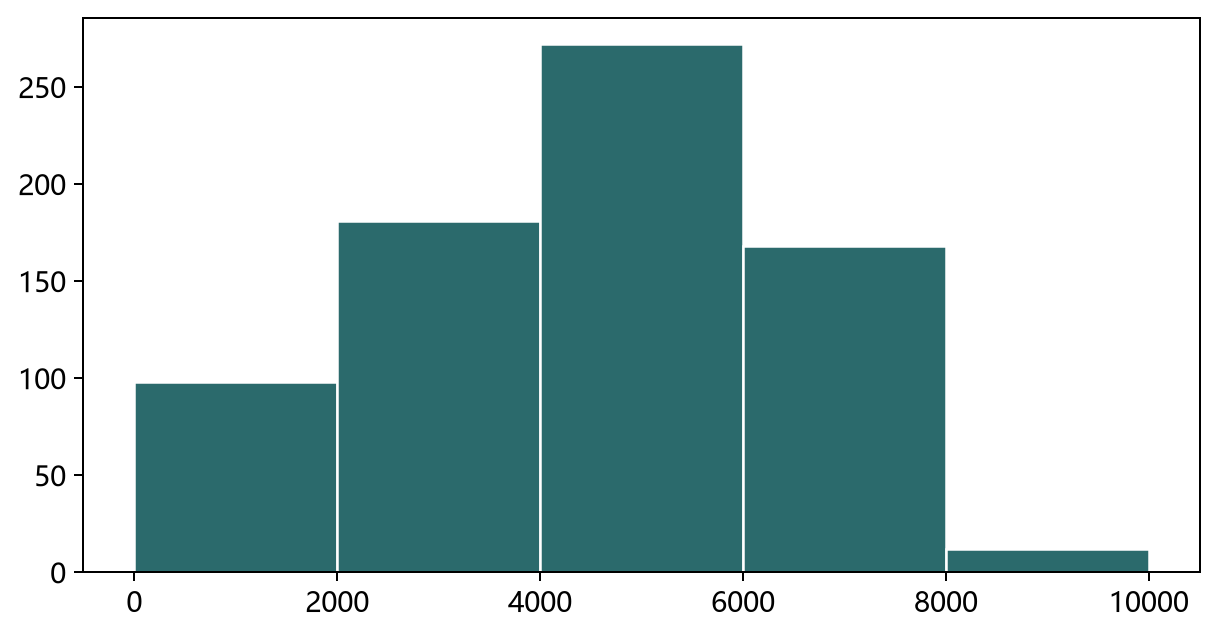
\includegraphics[width=\linewidth]{bike/hist_plain}
\end{column}
\begin{column}{.49\textwidth}\centering
\small 加上标题、单位、刻度和网格\\
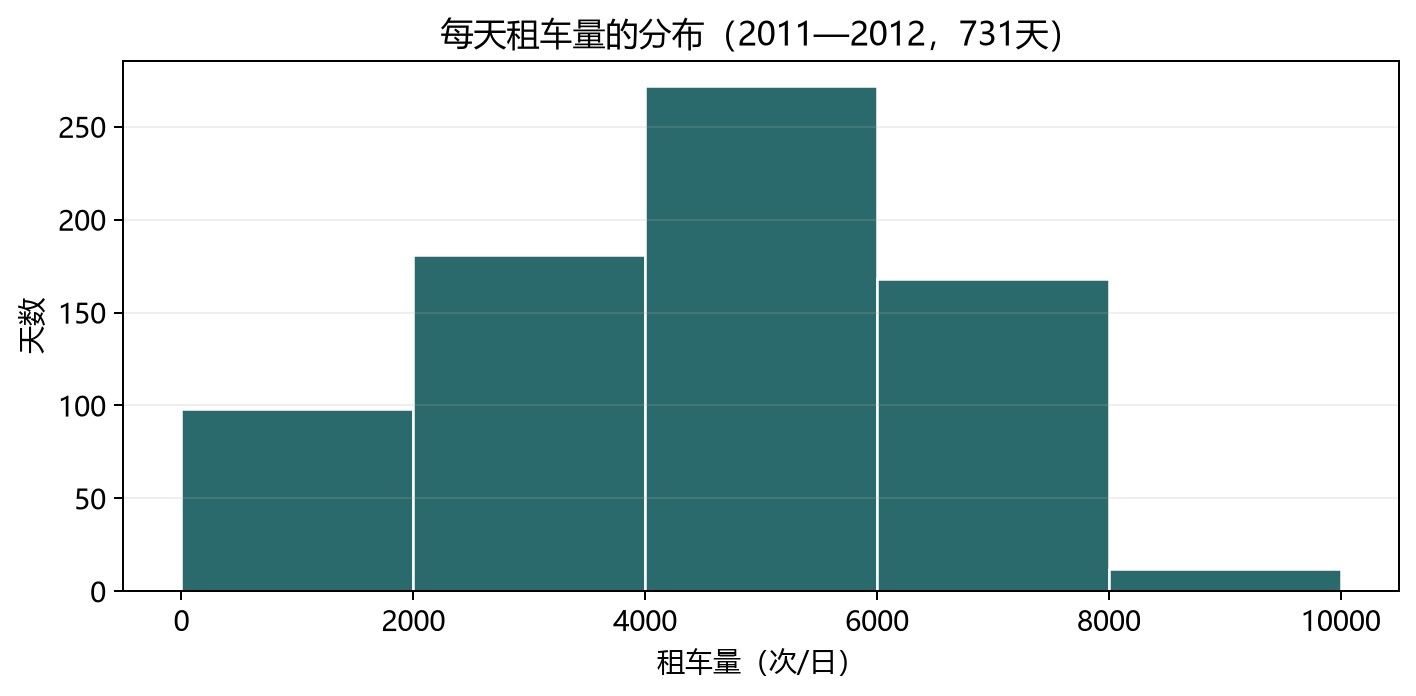
\includegraphics[width=\linewidth]{bike/hist_labeled}
\end{column}
\end{columns}
\medskip\small 从左到右，数据与分箱完全相同；标题和轴标签让读者知道“柱高数的是天，不是租车次数”。
\end{frame}

\begin{frame}{读图，再回到计数核对}
\begin{columns}[T,onlytextwidth]
\begin{column}{.40\textwidth}
\centering
\begin{tabular}{lr}
\toprule
租车次数区间 & 天数 \\
\midrule
$[0,2000)$ & 98 \\
$[2000,4000)$ & 181 \\
$[4000,6000)$ & 272 \\
$[6000,8000)$ & 168 \\
$[8000,10000]$ & 12 \\
\bottomrule
\end{tabular}
\end{column}
\begin{column}{.55\textwidth}
五根柱子的高度相加为 731 天。\par\medskip
最高一箱为 $[4000,6000)$，共有 272 天。\par\medskip
\texttt{bins} 决定边界；\texttt{hist} 自动数每一箱的观测。\par\medskip
除最后一箱外左闭右开，最后一箱包括右端点。
\end{column}
\end{columns}
\end{frame}

\begin{frame}[fragile]{bins 对照：只改变分箱数量}
\small 同样的 731 个值，共用横纵轴范围。这里用整数指定分箱数量，而不是手写分箱边界。\par\medskip
\begin{lstlisting}
fig, axes = plt.subplots(1, 3, figsize=(10, 3.5),
                         sharex=True, sharey=True)
for ax, bins in zip(axes, [10, 30, 60]):
    ax.hist(bike["cnt"], bins=bins,
            color="#2B6A6C", edgecolor="white")
    ax.set(title=f"bins={bins}", xlabel="租车量（次/日）")
axes[0].set_ylabel("天数")
fig.tight_layout()
plt.show()
\end{lstlisting}
\end{frame}

\begin{frame}{运行结果：bins 对照：只改变分箱数量}
\centering
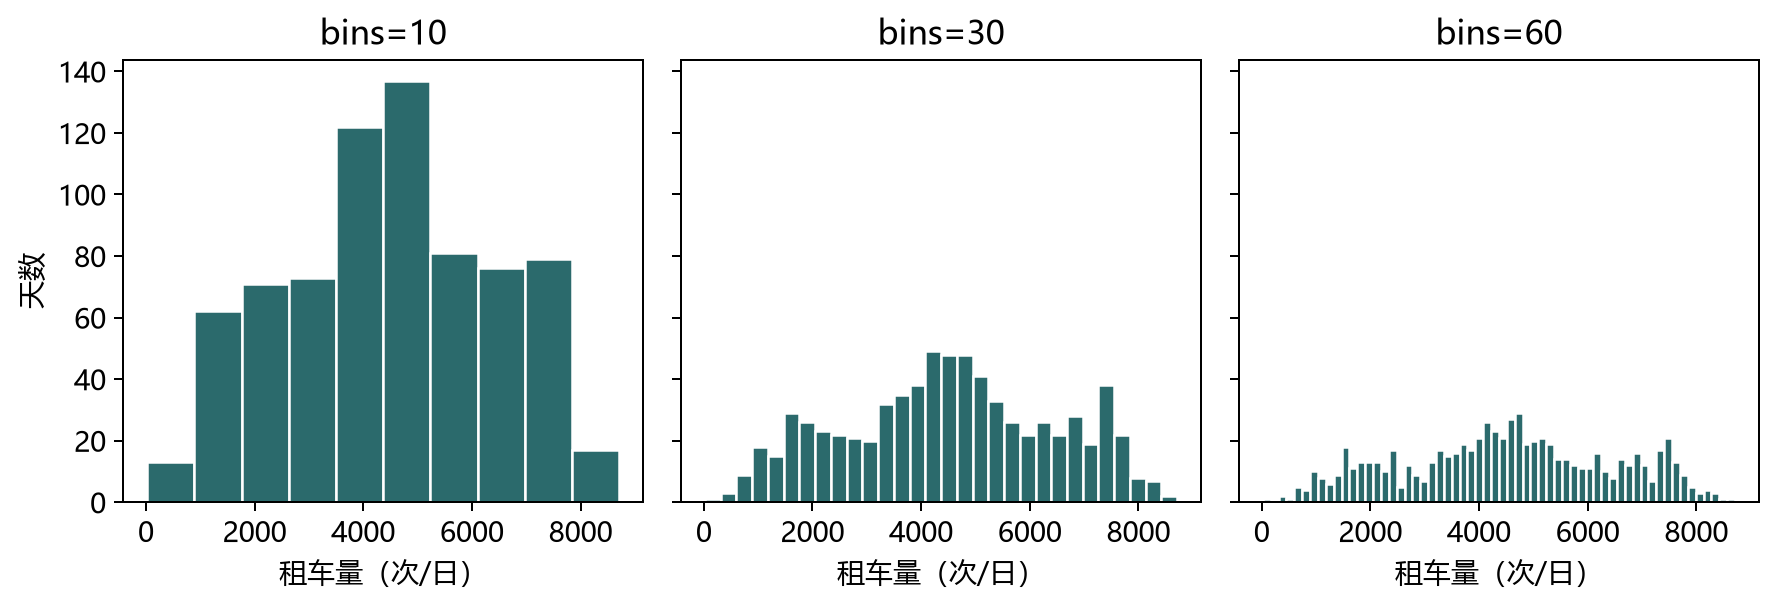
\includegraphics[width=.94\textwidth,height=.64\textheight,keepaspectratio]{bike/bins}
\par\medskip\small 箱数少会合并细节；箱数多会出现更细碎的起伏。数据没有改变，不能把分箱造成的变化当作新的事实。
\end{frame}

\begin{frame}[fragile]{density 对照：面积才代表比例}
\small 为便于读数，两图都把同一列除以 1000，单位改成千次/日；仍然是同一组记录。\par\medskip
\begin{lstlisting}
fig, axes = plt.subplots(1, 2, figsize=(9, 3.8))
for ax, density in zip(axes, [False, True]):
    ax.hist(bike["cnt"] / 1000, bins=np.array(bin_edges) / 1000,
            density=density, color="#2B6A6C", edgecolor="white")
    ax.set(title=f"density={density}", xlabel="租车量（千次/日）")
axes[0].set_ylabel("天数")
axes[1].set_ylabel("密度（每千次/日）")
fig.tight_layout()
plt.show()
\end{lstlisting}
\end{frame}

\begin{frame}{运行结果：density 对照：面积才代表比例}
\centering
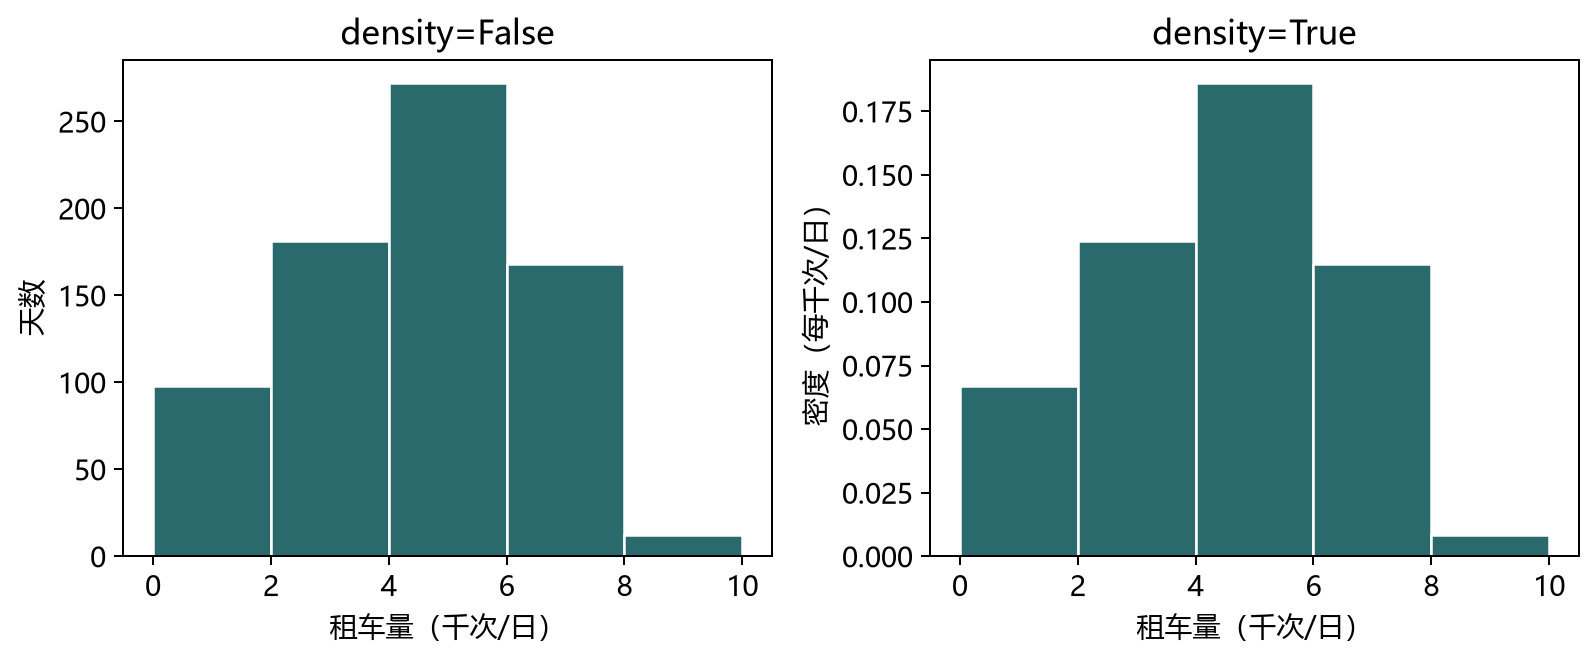
\includegraphics[width=.94\textwidth,height=.64\textheight,keepaspectratio]{bike/density}
\par\medskip\small 最高一箱宽度为 2：频数是 272，密度是 $272/(731\times2)\approx0.186$，面积约为 0.372，即 37.2\%。密度柱高不是概率。
\end{frame}

\section{柱状图：比较类别}

\begin{frame}[fragile]{工作日与非工作日，租车量有何不同？}
\small 分布图没有区分日类型。要比较工作日与非工作日，可用 workingday：1 表示既非周末又非节假日，0 表示其他日子。先求各组均值。\par\medskip
\begin{lstlisting}
work_summary = bike.groupby("workingday")["cnt"].agg(["mean", "size"])
work_labels = ["非工作日", "工作日"]
print(work_summary.round(1))
fig, ax = plt.subplots(figsize=(7, 4))
ax.bar(work_labels, work_summary["mean"], color="#2B6A6C")
ax.set(title="不同日类型的日均租车量（2011—2012）",
       xlabel="日类型", ylabel="平均租车量（次/日）", ylim=(0, 5500))
fig.tight_layout()
plt.show()
\end{lstlisting}
\end{frame}

\begin{frame}{运行结果：工作日与非工作日，租车量有何不同？}
\centering
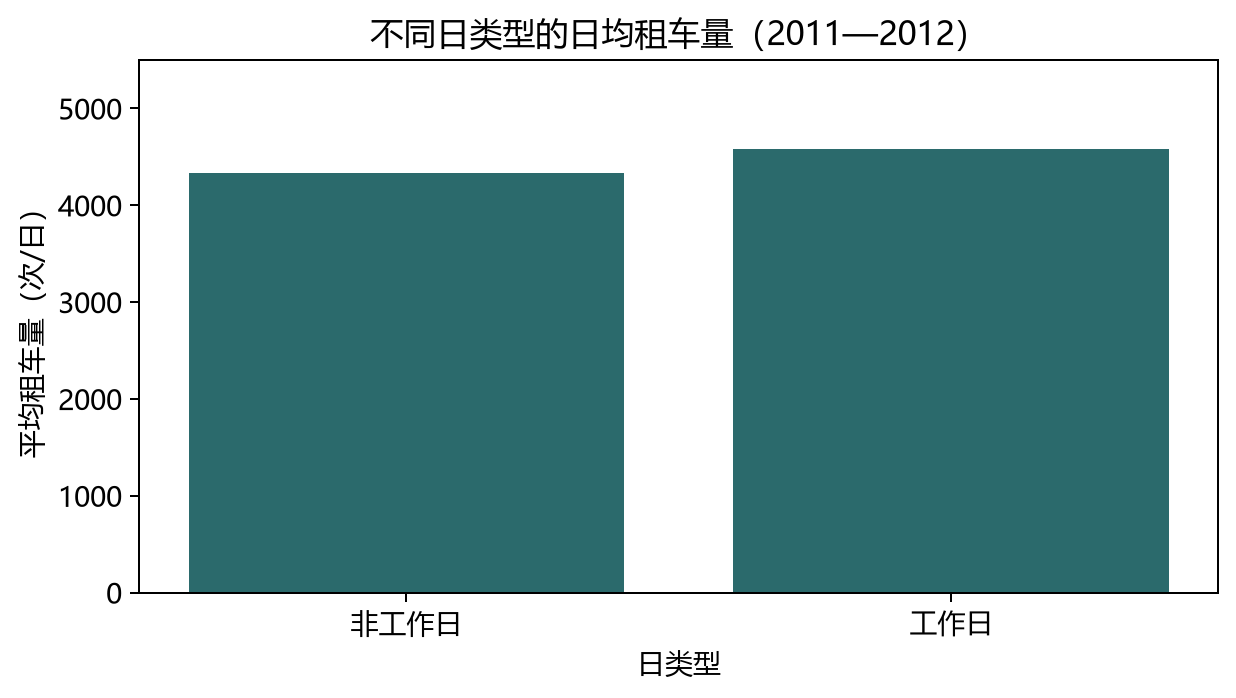
\includegraphics[width=.94\textwidth,height=.64\textheight,keepaspectratio]{bike/workbar}
\par\medskip\small 非工作日有 231 天，日均约 4330 次；工作日有 500 天，日均约 4585 次。两组天数不同，比较总次数会混入样本天数的影响。
\end{frame}

\begin{frame}[fragile]{bar 与 hist：两种柱子的含义}
\begin{lstlisting}
fig, axes = plt.subplots(1, 2, figsize=(10, 4))
axes[0].bar(work_labels, work_summary["mean"], color="#2B6A6C")
axes[0].set(title="bar：比较两个类别", ylabel="平均租车量（次/日）")
axes[1].hist(bike["cnt"], bins=bin_edges,
             color="#2B6A6C", edgecolor="white")
axes[1].set(title="hist：统计数值区间", xlabel="租车量（次/日）", ylabel="天数")
fig.tight_layout()
plt.show()
\end{lstlisting}
\end{frame}

\begin{frame}{运行结果：bar 与 hist：两种柱子的含义}
\centering
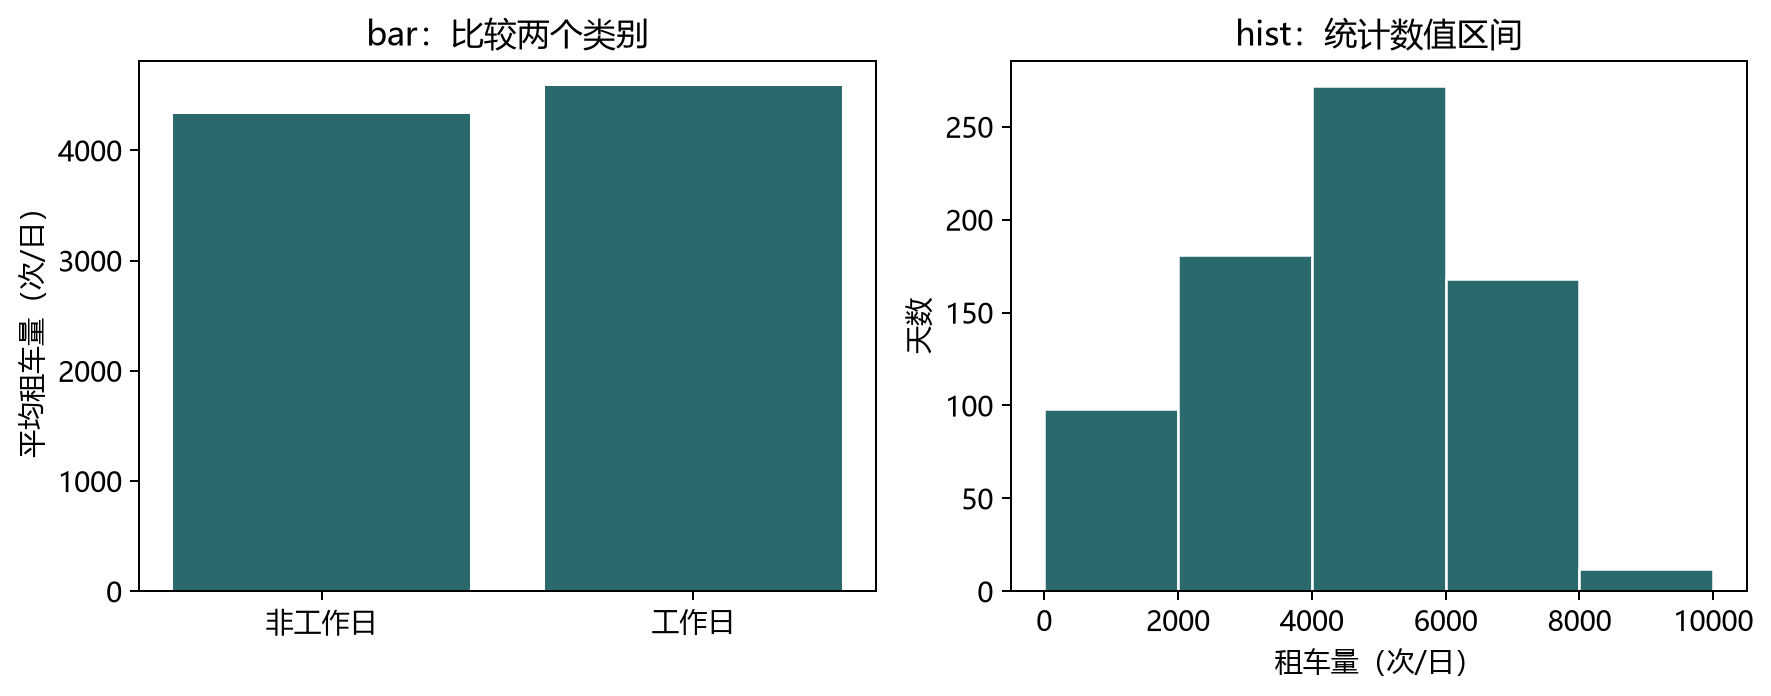
\includegraphics[width=.94\textwidth,height=.64\textheight,keepaspectratio]{bike/bar_vs_hist}
\par\medskip\small 左边输入“类别与算好的均值”，每根柱子对应一类日子；右边输入原始 cnt，自动分箱，每根柱子对应一个租车量区间。
\end{frame}

\begin{frame}{课堂练习：只有两根柱子，信息够吗？}
\begin{enumerate}
\item 两组均值接近，是否说明每一天的租车量都接近？
\item 两类日子的总量接近，是否说明用户构成也一样？
\item 如果先用 \texttt{sum()} 再画柱状图，纵轴该写什么单位？
\end{enumerate}
\begin{block}{先保留问题}
均值只能概括平均水平。判断每天是否相似，要看分布；判断用户构成是否相似，需要区分用户类型。
\end{block}
\end{frame}

\section{折线图与面积图}

\begin{frame}[fragile]{租车量随时间如何变化？}
\small 前面的分布和均值没有显示时间顺序。要看租车量何时高、何时低，需要用日期 dteday 作横轴，并按日期排序。\par\medskip
\begin{lstlisting}
fig, ax = plt.subplots(figsize=(9, 4))
ax.plot(bike["dteday"], bike["cnt"],
        color="#2B6A6C", linewidth=0.9)
ax.set(title="每日租车量（2011—2012，731天）",
       xlabel="日期", ylabel="租车量（次/日）")
ax.grid(alpha=0.2)
fig.tight_layout()
plt.show()
\end{lstlisting}
\end{frame}

\begin{frame}{运行结果：租车量随时间如何变化？}
\centering
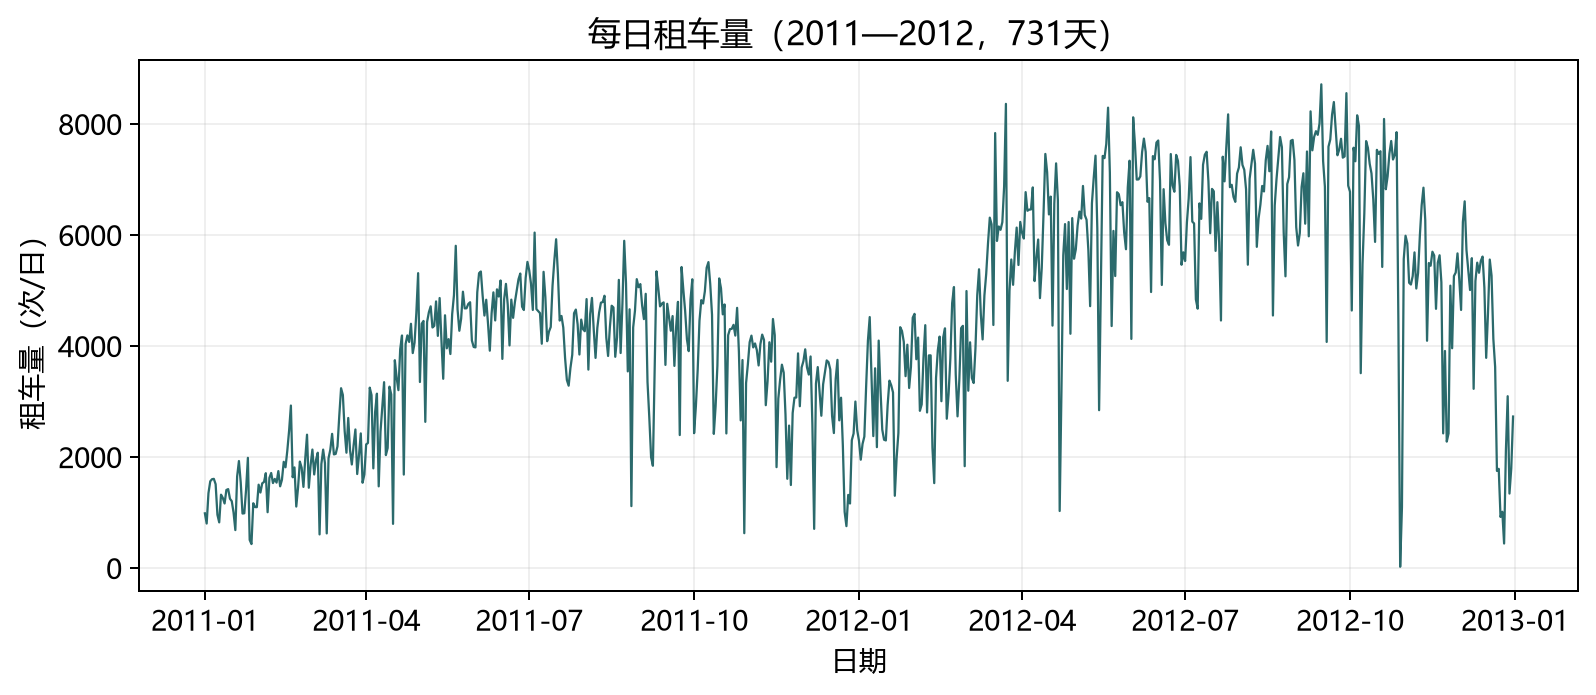
\includegraphics[width=.94\textwidth,height=.64\textheight,keepaspectratio]{bike/daily}
\par\medskip\small 横轴是日期，纵轴仍是 cnt；连线表示相邻日期。两年中都有起伏，单个高低点的原因不能只凭这张图认定。
\end{frame}

\begin{frame}[fragile]{每天波动很大，怎样看清月度变化？}
\small 每日曲线起伏较多，可以先看每个月的平均水平。resample("MS") 按月分组，mean() 求月内日均值，得到 24 个点。\par\medskip
\begin{lstlisting}
monthly = bike.set_index("dteday").resample("MS")["cnt"].mean()
fig, ax = plt.subplots(figsize=(9, 4))
ax.plot(monthly.index, monthly, color="#2B6A6C",
        marker="o", linewidth=2, label="月内日均租车量")
ax.set(title="月内日均租车量（2011—2012，24个月）",
       xlabel="月份", ylabel="月内平均租车量（次/日）")
ax.legend()
ax.grid(alpha=0.2)
fig.tight_layout()
plt.show()
\end{lstlisting}
\end{frame}

\begin{frame}{运行结果：每天波动很大，怎样看清月度变化？}
\centering
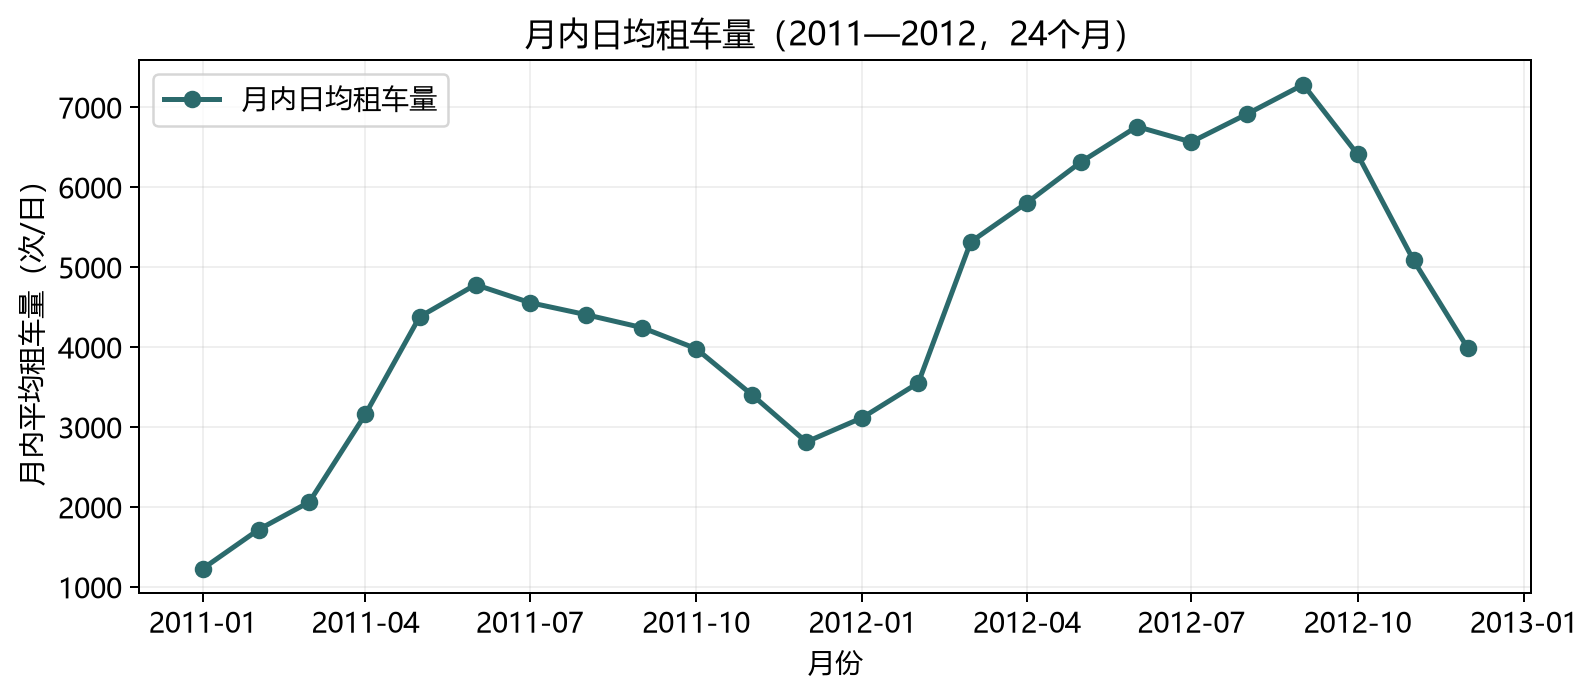
\includegraphics[width=.94\textwidth,height=.64\textheight,keepaspectratio]{bike/monthly}
\par\medskip\small marker="o" 标出 24 个月；label 提供图例文字，legend() 显示图例。月均值减少每日波动，不能读作月度总次数。
\end{frame}

\begin{frame}[fragile]{样式对照：只取原表前七天}
\small 用前七天的租车记录观察线条样式。每幅只改变一个参数，便于对应代码与效果。\par\medskip
\begin{lstlisting}
week = bike.head(7)
styles = [{}, {"color": "#B40D49"}, {"linestyle": "--"},
          {"marker": "o"}, {"linewidth": 4}, {"alpha": 0.25}]
titles = ["默认", "color", "linestyle='--'", "marker='o'",
          "linewidth=4", "alpha=0.25"]
fig, axes = plt.subplots(2, 3, figsize=(10, 5), sharex=True, sharey=True)
for ax, style, title in zip(axes.flat, styles, titles):
    ax.plot(week["dteday"].dt.day, week["cnt"], **style)
    ax.set(title=title, xticks=[1, 3, 5, 7])
fig.supxlabel("2011年1月的日期")
fig.supylabel("租车量（次/日）")
fig.tight_layout()
plt.show()
\end{lstlisting}
\end{frame}

\begin{frame}{运行结果：样式对照：只取原表前七天}
\centering
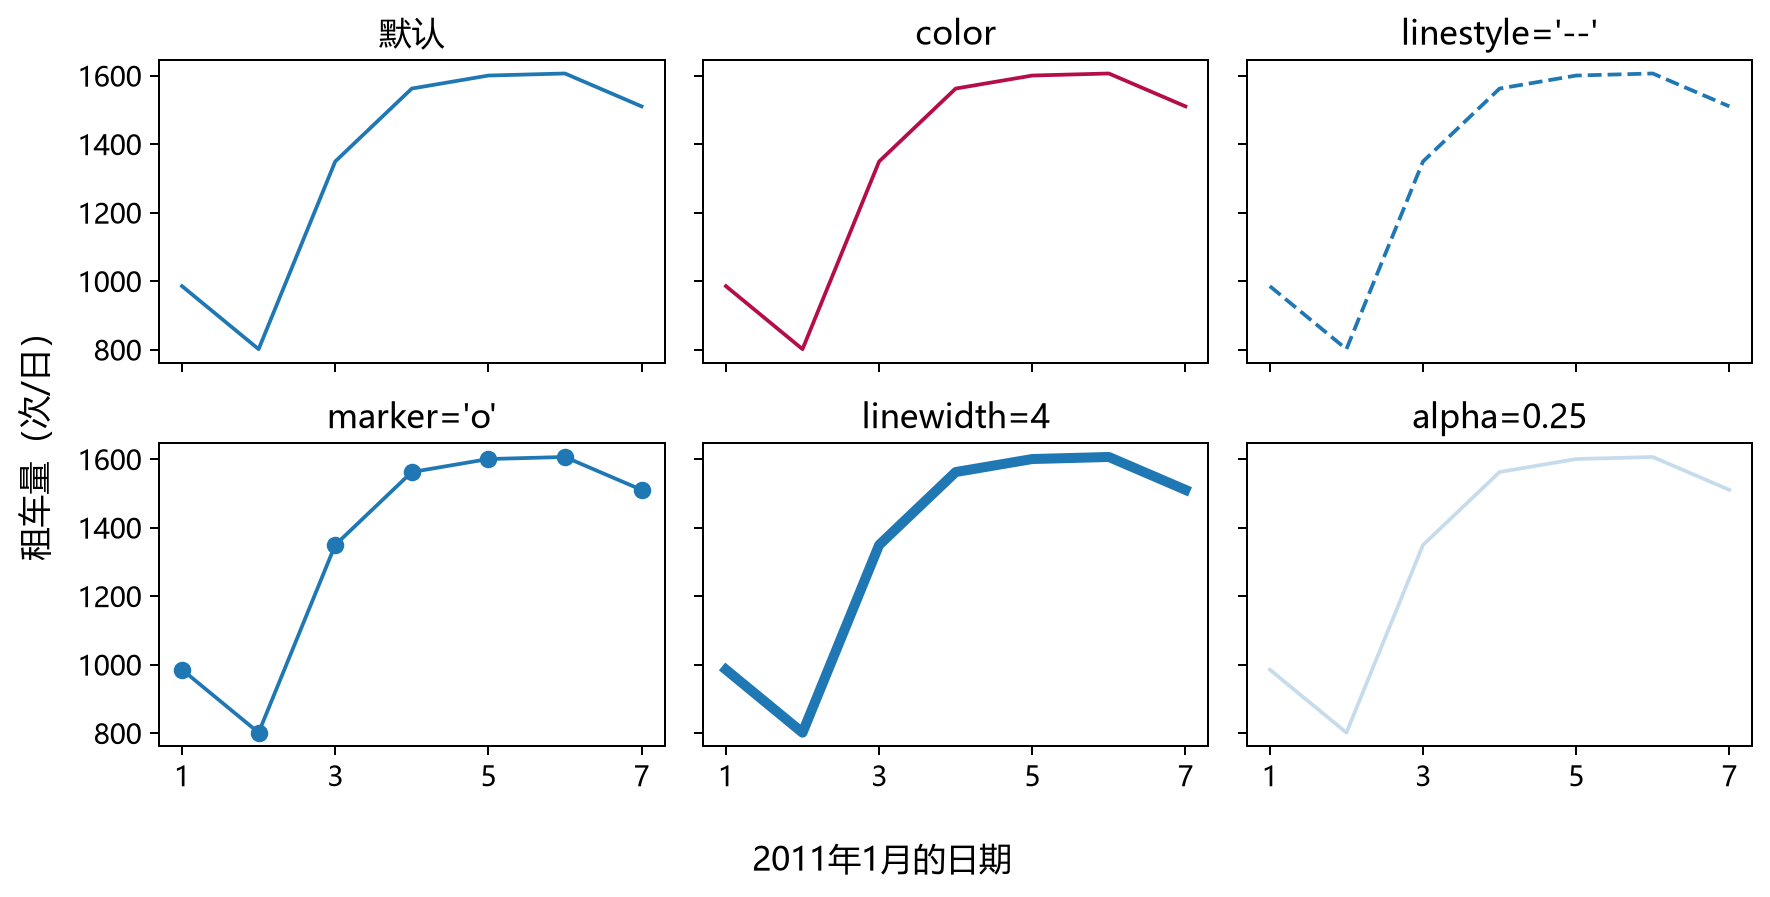
\includegraphics[width=.94\textwidth,height=.64\textheight,keepaspectratio]{bike/styles}
\par\medskip\small 颜色、虚线、圆点、粗细、透明度分别由一个参数控制。实际画图时可以把这些参数组合起来；参数改变外观，不改变原始值。
\end{frame}

\begin{frame}[fragile]{两类用户的租车量如何变化？}
\small 总量的变化来自哪些用户？casual 记录临时用户租车次数，registered 记录注册用户租车次数；两类之和等于 cnt。分别画线可以比较各自的变化。\par\medskip
\begin{lstlisting}
user_monthly = bike.set_index("dteday").resample("MS")[["casual", "registered", "cnt"]].mean()
fig, ax = plt.subplots(figsize=(9, 4))
ax.plot(user_monthly.index, user_monthly["casual"],
        color="#B40D49", linestyle="--", label="临时用户")
ax.plot(user_monthly.index, user_monthly["registered"],
        color="#2B6A6C", label="注册用户")
ax.set(title="两类用户的月内日均租车量（2011—2012）",
       xlabel="月份", ylabel="平均租车量（次/日）")
ax.legend()
fig.tight_layout()
plt.show()
\end{lstlisting}
\end{frame}

\begin{frame}{运行结果：两类用户的租车量如何变化？}
\centering
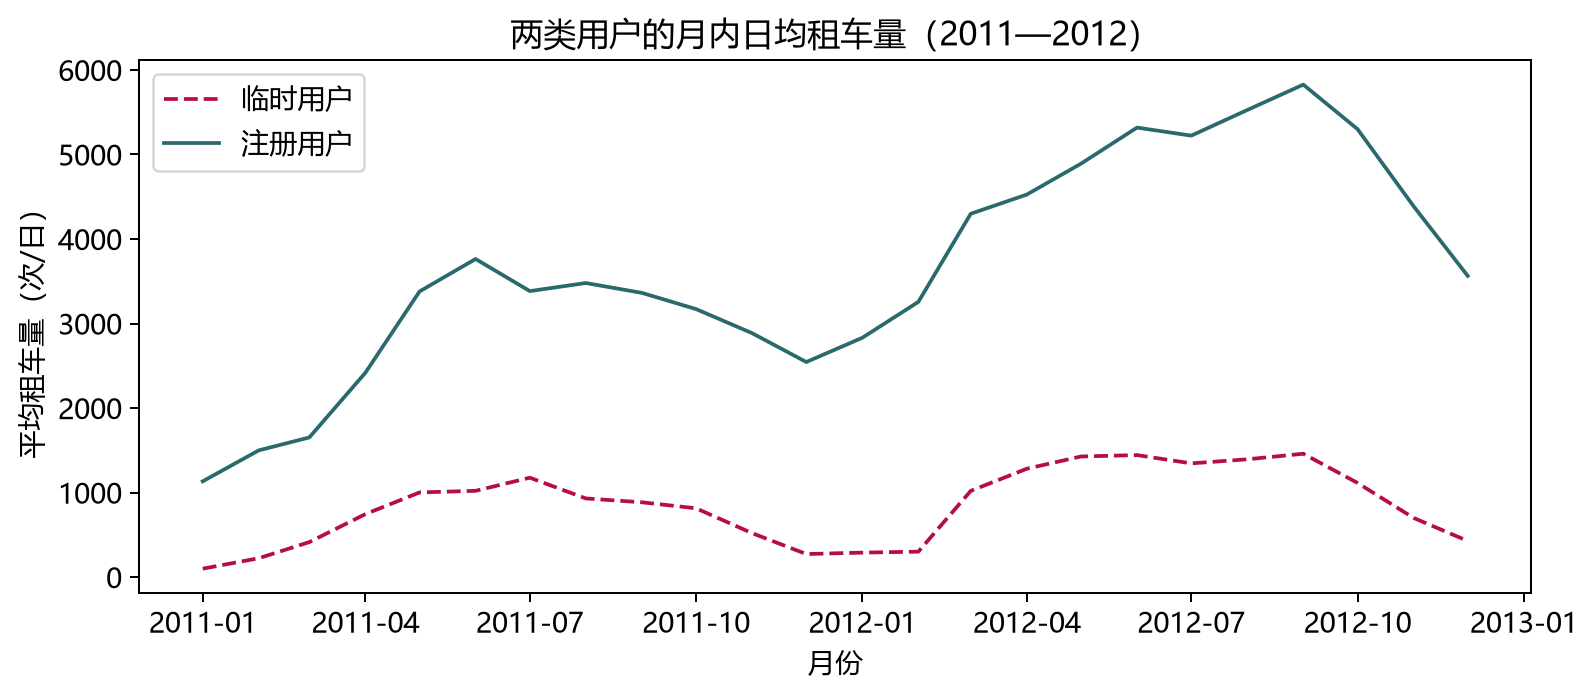
\includegraphics[width=.94\textwidth,height=.64\textheight,keepaspectratio]{bike/users}
\par\medskip\small 每次 plot 增加一条线；实线与虚线也能区分类别。两条曲线仍来自同样的 24 个月，纵轴单位一致。
\end{frame}

\begin{frame}[fragile]{总量接近，用户构成也一样吗？}
\small 工作日与非工作日的日均总量接近，两类用户是否也如此？分别计算各组的临时、注册用户日均租车量，用并排的柱子比较。\par\medskip
\begin{lstlisting}
user_work = bike.groupby("workingday")[["casual", "registered"]].mean()
x = np.arange(2)
fig, ax = plt.subplots(figsize=(7, 4))
ax.bar(x - 0.18, user_work["casual"], width=0.36,
       color="#B40D49", label="临时用户")
ax.bar(x + 0.18, user_work["registered"], width=0.36,
       color="#2B6A6C", label="注册用户")
ax.set_xticks(x, work_labels)
ax.set(title="按日类型拆开用户构成（2011—2012）", ylabel="平均租车量（次/日）")
ax.legend()
fig.tight_layout()
plt.show()
\end{lstlisting}
\end{frame}

\begin{frame}{运行结果：总量接近，用户构成也一样吗？}
\centering
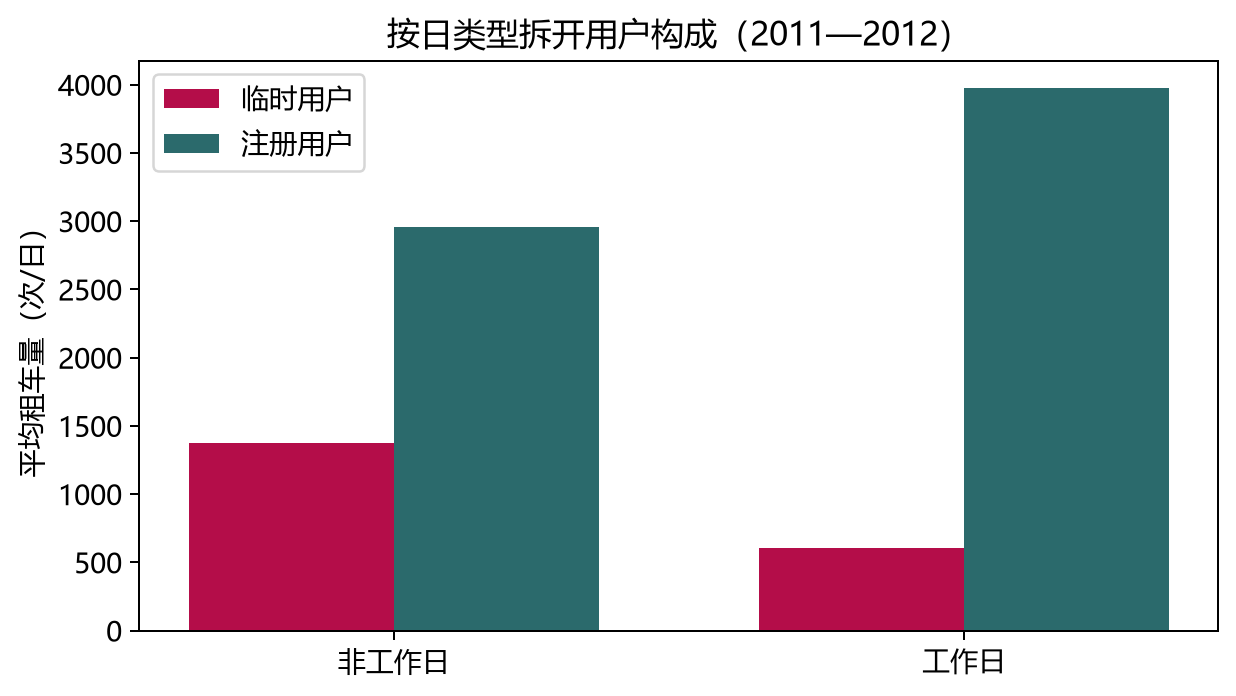
\includegraphics[width=.94\textwidth,height=.64\textheight,keepaspectratio]{bike/grouped_bar}
\par\medskip\small 临时用户：非工作日约 1371 次/日，工作日约 607；注册用户：约 2959 与 3978。总量接近可以掩盖构成差异；图本身不能证明出行目的。
\end{frame}

\begin{frame}[fragile]{fill\_between：两条边界之间填充}
\small 下层从 0 填到 registered，上层从 registered 填到 cnt。上下两层的厚度分别对应两类租车量。\par\medskip
\begin{lstlisting}
fig, ax = plt.subplots(figsize=(9, 4))
ax.fill_between(user_monthly.index, 0, user_monthly["registered"],
                color="#2B6A6C", alpha=0.6, label="注册用户")
ax.fill_between(user_monthly.index, user_monthly["registered"],
                user_monthly["cnt"], color="#B40D49", alpha=0.45, label="临时用户")
ax.set(title="月内日均租车量的构成（2011—2012）",
       xlabel="月份", ylabel="平均租车量（次/日）", ylim=(0, 8000))
ax.legend()
fig.tight_layout()
plt.show()
\end{lstlisting}
\end{frame}

\begin{frame}{运行结果：fill\_between：两条边界之间填充}
\centering
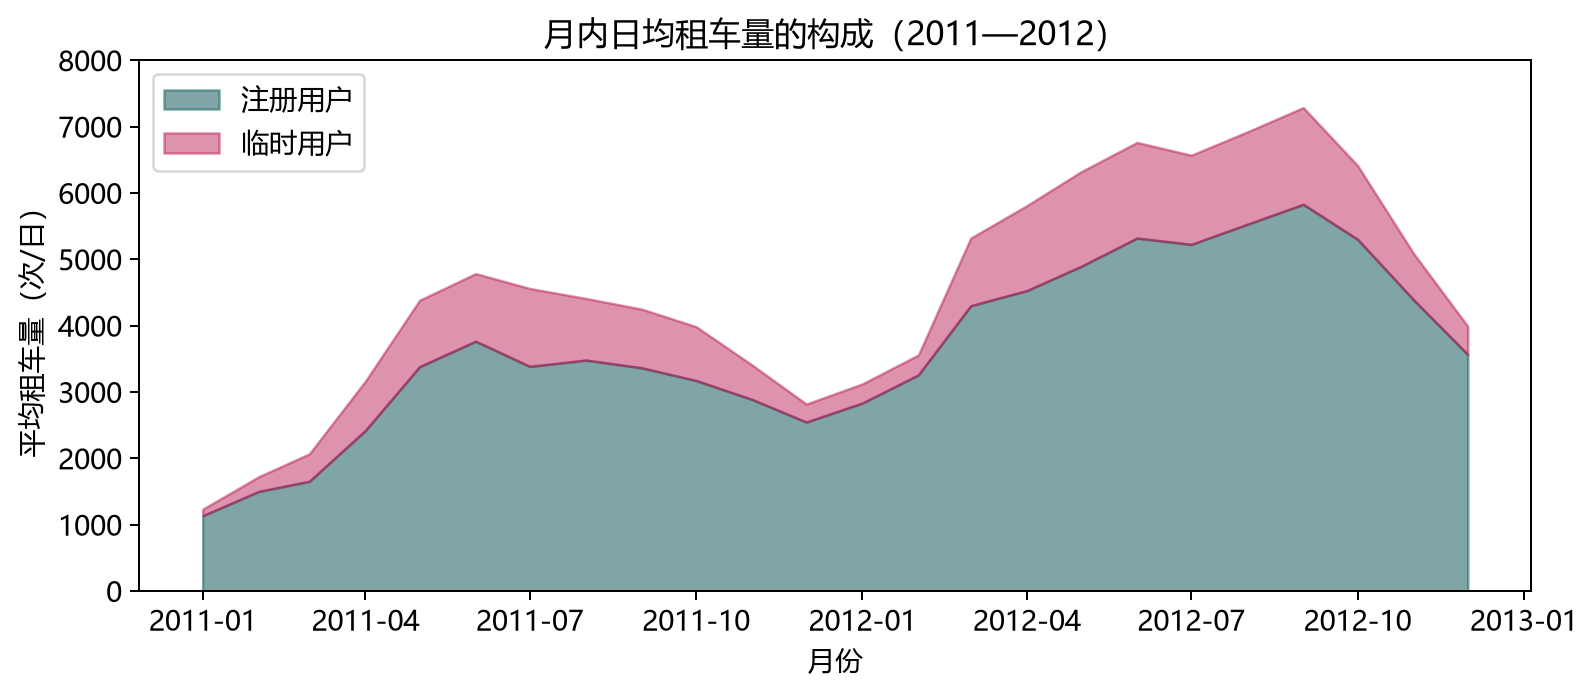
\includegraphics[width=.94\textwidth,height=.64\textheight,keepaspectratio]{bike/area}
\par\medskip\small fill\_between(x, y1, y2) 填充两条边界之间的区域；alpha 控制透明度。最上方边界是总量，上层厚度才是临时用户量。
\end{frame}

\section{散点图：观察关系}

\begin{frame}[fragile]{天气暖和时，租车量会更高吗？}
\small 租车量的起伏是否与温度有关？用标准化温度 temp 与同一天的 cnt 配成一个点，观察二者的关系。temp 不是摄氏度。\par\medskip
\begin{lstlisting}
fig, ax = plt.subplots(figsize=(7, 4.5))
ax.scatter(bike["temp"], bike["cnt"],
           color="#2B6A6C", alpha=0.45, s=22)
ax.set(title="温度与每日租车量（2011—2012，731天）",
       xlabel="标准化温度 temp（无量纲）", ylabel="租车量（次/日）")
ax.grid(alpha=0.2)
fig.tight_layout()
plt.show()
\end{lstlisting}
\end{frame}

\begin{frame}{运行结果：天气暖和时，租车量会更高吗？}
\centering
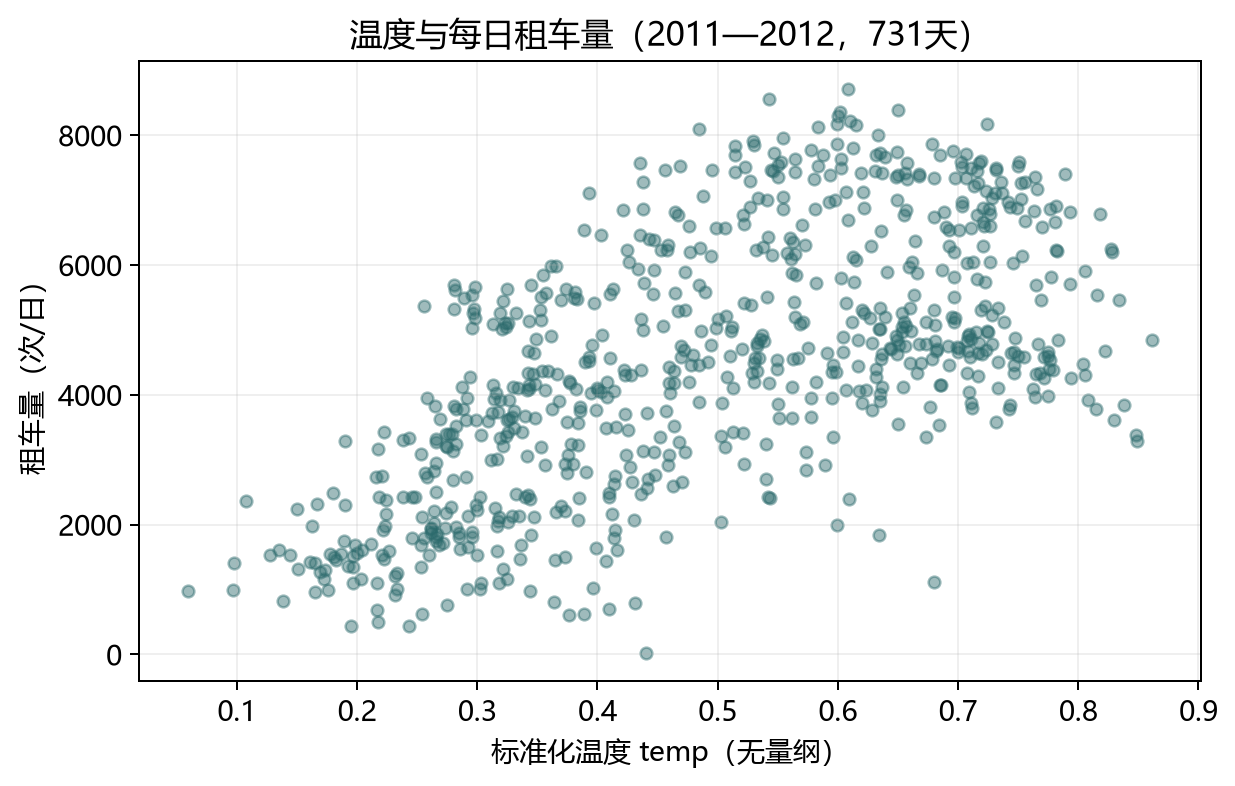
\includegraphics[width=.94\textwidth,height=.64\textheight,keepaspectratio]{bike/scatter}
\par\medskip\small 每个点代表一天。较暖的日子总体对应较高租车量，但同一温度附近仍有很大差异。alpha 减少重叠遮挡，s 控制点的面积。
\end{frame}

\begin{frame}[fragile]{相近温度下，两年的租车量一样吗？}
\small 相近温度下，租车量仍有很大差异，会不会与年份有关？用 yr 区分 2011（0）与 2012（1），以颜色和点形标记，横纵轴保持不变。\par\medskip
\begin{lstlisting}
fig, ax = plt.subplots(figsize=(7, 4.5))
for year, color, marker in [(0, "#2B6A6C", "o"), (1, "#B40D49", "^")]:
    part = bike[bike["yr"] == year]
    ax.scatter(part["temp"], part["cnt"], color=color,
               marker=marker, alpha=0.5, s=24, label=str(2011 + year))
ax.set(title="按年份区分温度与租车量（2011—2012）",
       xlabel="标准化温度 temp（无量纲）", ylabel="租车量（次/日）")
ax.legend()
fig.tight_layout()
plt.show()
\end{lstlisting}
\end{frame}

\begin{frame}{运行结果：相近温度下，两年的租车量一样吗？}
\centering
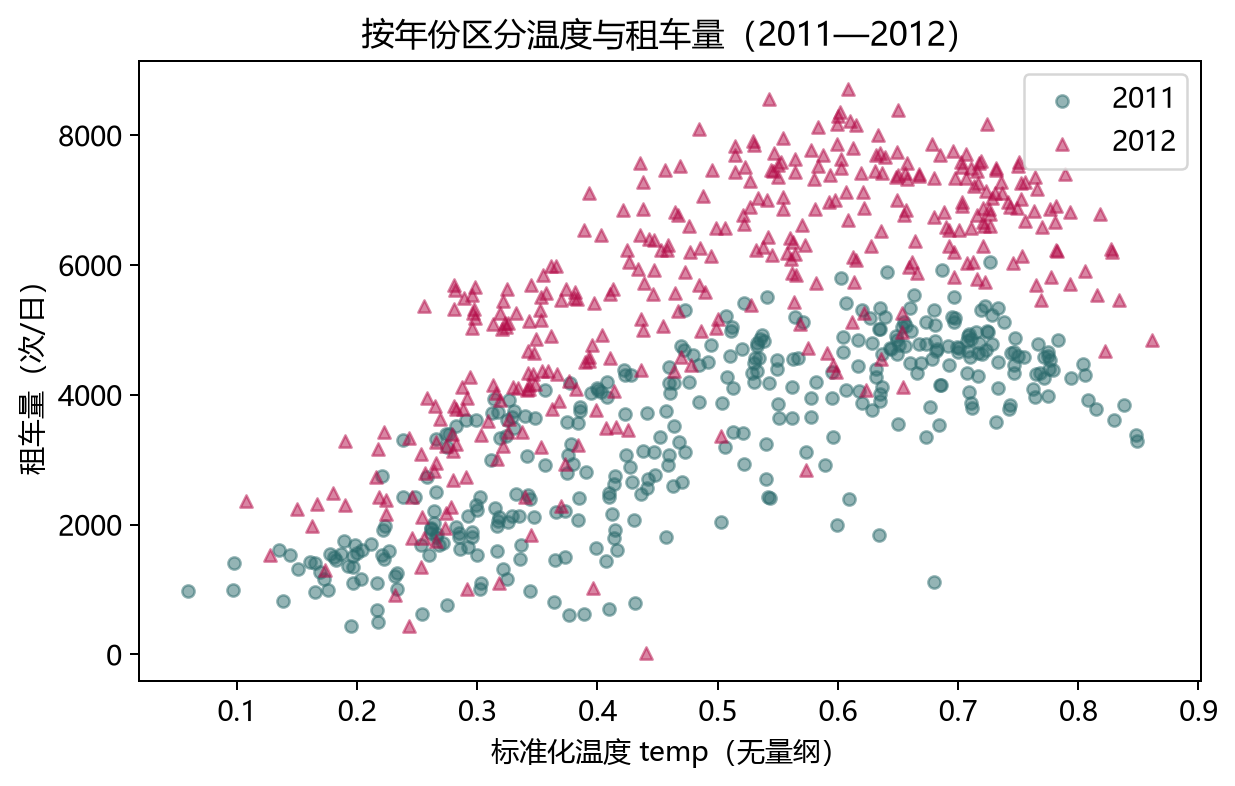
\includegraphics[width=.94\textwidth,height=.64\textheight,keepaspectratio]{bike/scatter_year}
\par\medskip\small 2012 年的点群整体偏高；同一张无分组散点图混合了年份差异。分组展示有助于发现结构，但没有控制所有影响因素，也不能据此确定因果。
\end{frame}

\begin{frame}{除了温度，还有什么可能与租车量有关？}
\begin{itemize}
\item \texttt{hum}：标准化湿度，可乘 100 表示百分比。
\item \texttt{weathersit}：天气类别，日表实际出现 1、2、3。
\item \texttt{workingday}：工作日结构可能与租车行为相关。
\end{itemize}
\begin{block}{下一步可以研究什么？}
湿度较高时，租车量是否不同？不同天气类别之间是否有差异？根据具体问题选择散点图、分组比较或子图。
\end{block}
\small 本章做描述性探索；季节、年份、天气等因素可能同时变化，图形关系不自动等于因果关系。
\end{frame}

\section{图形布局与保存}

\begin{frame}[fragile]{subplots：上下两图共享日期轴}
\small 2, 1 表示两行一列。axes[0] 在上，axes[1] 在下；sharex=True 共享月份范围。\par\medskip
\begin{lstlisting}
fig, axes = plt.subplots(2, 1, figsize=(9, 5), sharex=True)
axes[0].plot(user_monthly.index, user_monthly["cnt"], color="#2B6A6C")
axes[0].set(title="总租车量", ylabel="平均租车量（次/日）")
axes[1].plot(user_monthly.index, user_monthly["casual"], color="#B40D49")
axes[1].set(title="其中：临时用户租车量", xlabel="月份", ylabel="平均租车量（次/日）")
fig.suptitle("月内日均租车量（2011—2012）")
fig.tight_layout()
plt.show()
\end{lstlisting}
\end{frame}

\begin{frame}{运行结果：subplots：上下两图共享日期轴}
\centering
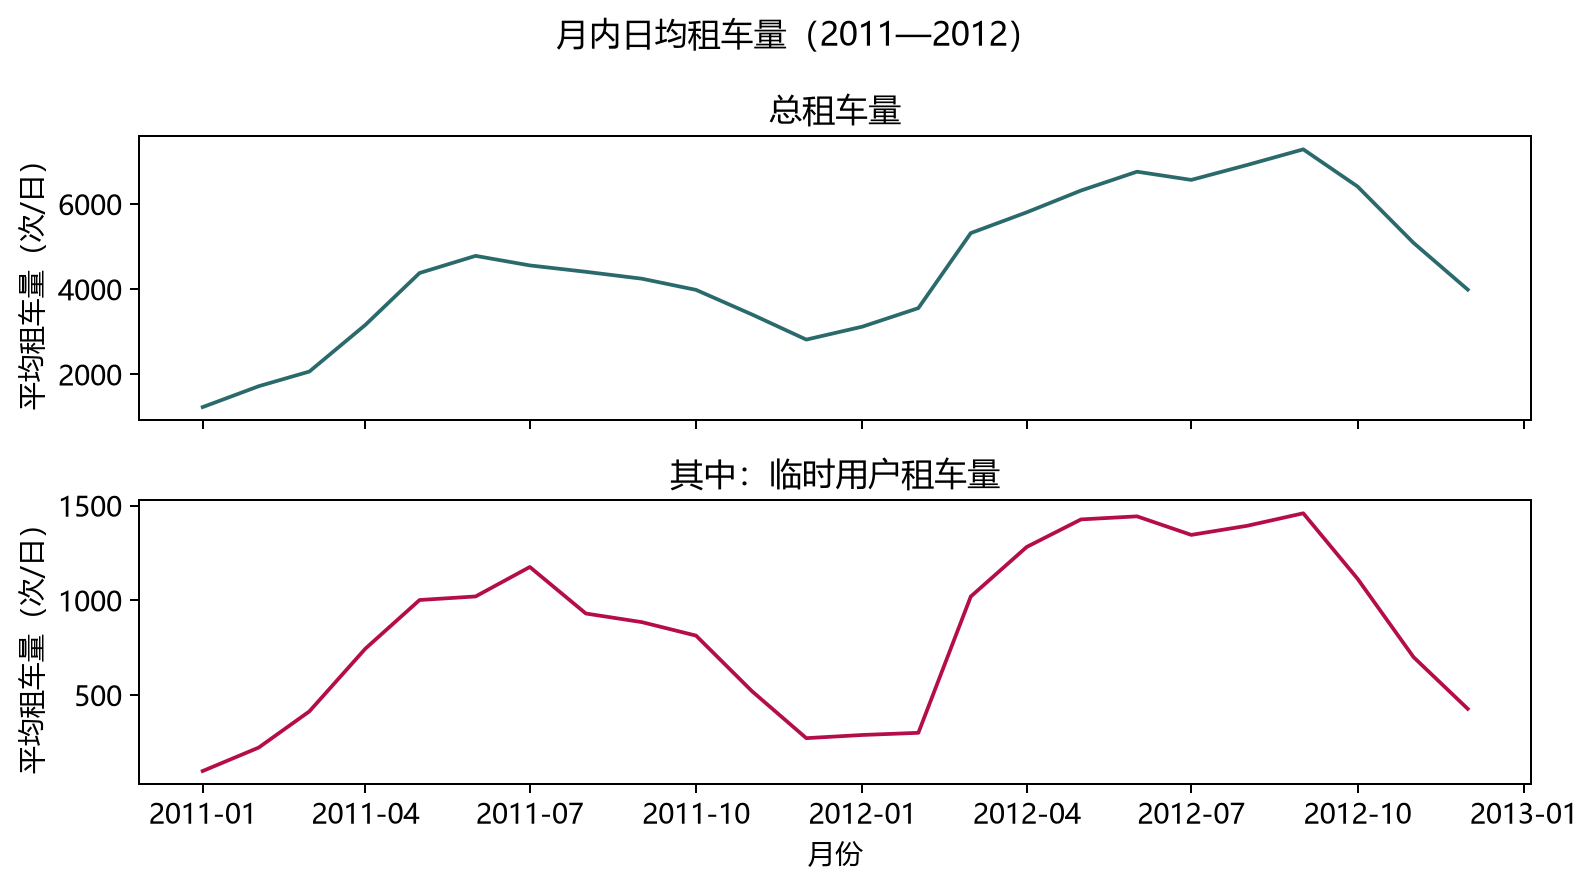
\includegraphics[width=.94\textwidth,height=.64\textheight,keepaspectratio]{bike/subplots}
\par\medskip\small 上图隐藏重复的日期文字，下图保留；tight\_layout() 调整间距。两幅图纵轴范围不同，比较数值时仍要读刻度。
\end{frame}

\begin{frame}[fragile]{用 pandas 快速画出两条曲线}
\small DataFrame.plot 默认把索引作为横轴、每列作为一条线。返回的仍是 Matplotlib 坐标系。\par\medskip
\begin{lstlisting}
ax = user_monthly[["casual", "registered"]].plot(
    figsize=(9, 4), color=["#B40D49", "#2B6A6C"],
    style=["--", "-"], grid=True)
ax.set(title="pandas 快捷绘图：两类用户（2011—2012）",
       xlabel="月份", ylabel="月内平均租车量（次/日）")
ax.legend(["临时用户", "注册用户"])
fig = ax.figure
fig.tight_layout()
plt.show()
\end{lstlisting}
\end{frame}

\begin{frame}{运行结果：用 pandas 快速画出两条曲线}
\centering
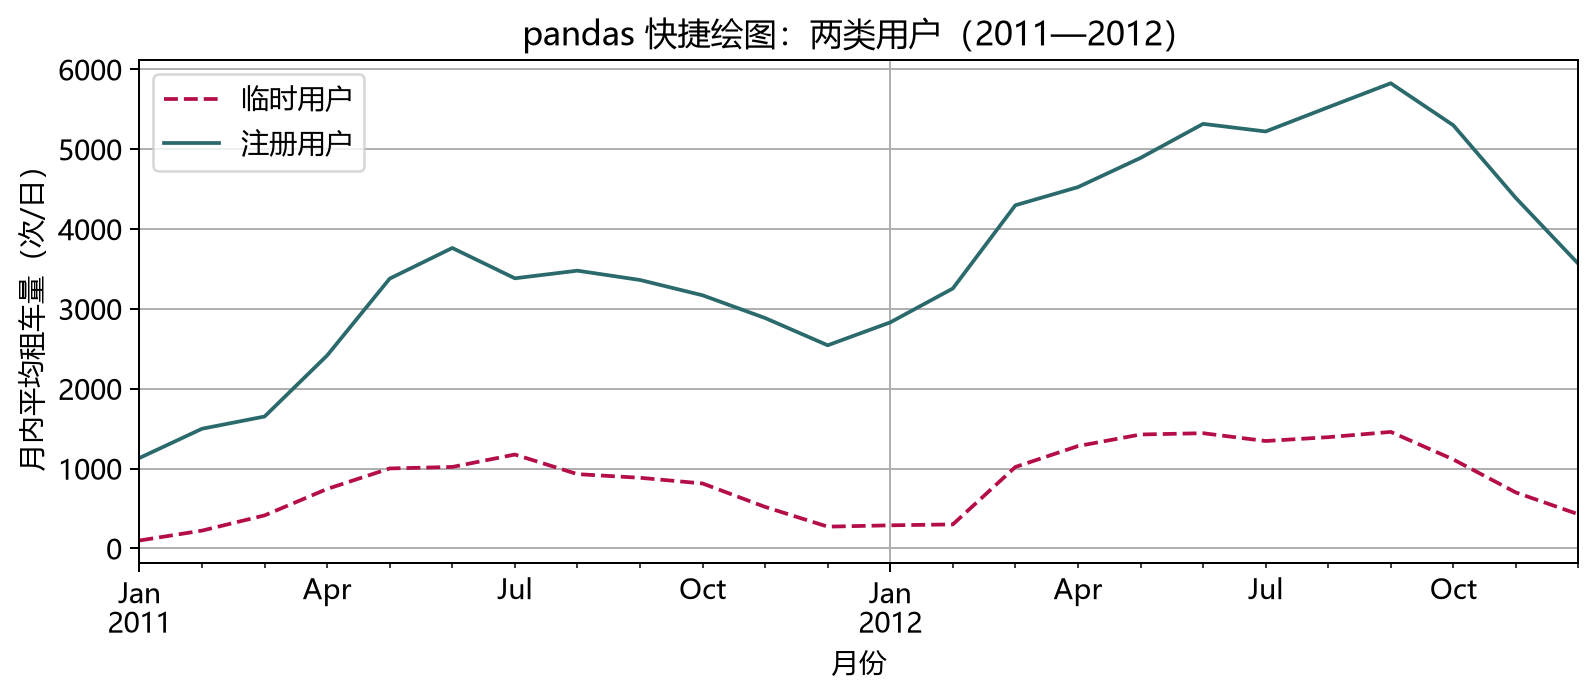
\includegraphics[width=.94\textwidth,height=.64\textheight,keepaspectratio]{bike/pandas}
\par\medskip\small 这与前面的两条用户曲线使用完全相同的数据。探索时可以使用 pandas 快捷接口，需要细调时继续调用 ax 的方法。
\end{frame}

\begin{frame}[fragile]{综合图（上）：先放时间与类别比较}
\small axes[行, 列] 从 0 开始。先完成上面一行；接着运行下一页代码，填满同一张画布。\par\medskip
\begin{lstlisting}
fig, axes = plt.subplots(2, 2, figsize=(11, 7))
axes[0, 0].plot(monthly.index, monthly, color="#2B6A6C")
axes[0, 0].set(title="月内日均租车量", xlabel="月份", ylabel="次/日")
tick_dates = monthly.index[[0, 6, 12, 18, 23]]
axes[0, 0].set_xticks(tick_dates, tick_dates.strftime("%Y-%m"))
axes[0, 1].bar(work_labels, work_summary["mean"], color="#2B6A6C")
axes[0, 1].set(title="日类型比较", ylabel="平均租车量（次/日）")
plt.close(fig)  # 暂不显示，下一单元格继续完成
\end{lstlisting}
\end{frame}

\begin{frame}[fragile]{综合图（下）：再放分布与关系}
\begin{lstlisting}
axes[1, 0].hist(bike["cnt"], bins=bin_edges,
                color="#2B6A6C", edgecolor="white")
axes[1, 0].set(title="每日租车量分布", xlabel="次/日", ylabel="天数")
axes[1, 1].scatter(bike["temp"], bike["cnt"],
                   color="#2B6A6C", alpha=0.4, s=10)
axes[1, 1].set(title="温度与每日租车量", xlabel="标准化温度", ylabel="次/日")
fig.suptitle("同一张日表的四个视角（2011—2012，731天）")
fig.tight_layout()
display(fig)  # 显示前一单元格创建、现已完成的画布
\end{lstlisting}
\end{frame}

\begin{frame}{运行结果：综合图（下）：再放分布与关系}
\centering
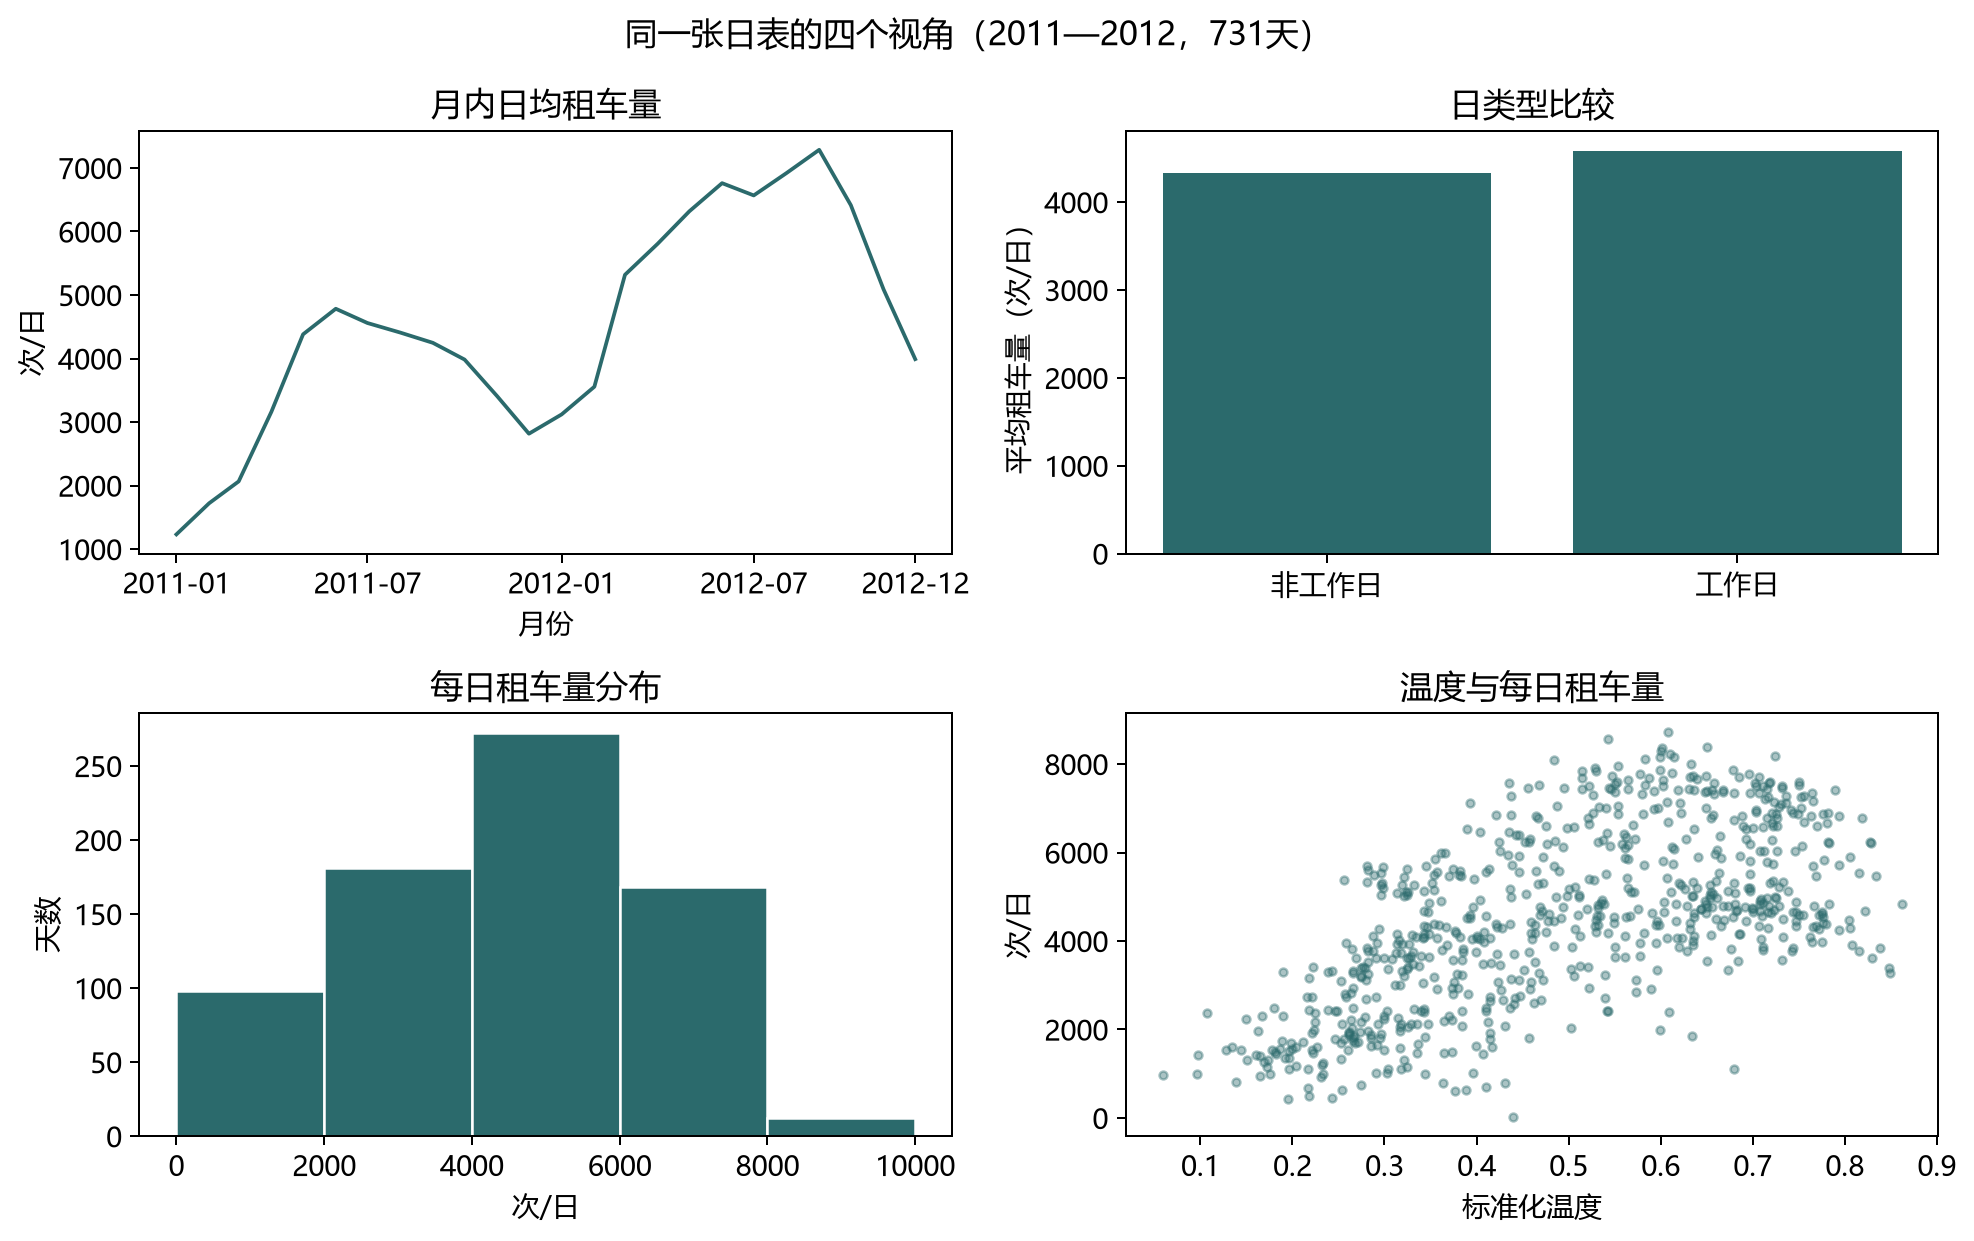
\includegraphics[width=.94\textwidth,height=.64\textheight,keepaspectratio]{bike/report}
\par\medskip\small 左上是时间，右上是类别，左下是分布，右下是关系。四幅图来自同一张表，但统计单位与纵轴含义并不完全相同。
\end{frame}

\begin{frame}[fragile]{保存图片：导出刚才的四宫格}
\small fig 保留对刚才画布的引用。文件名后缀决定 PNG 或 PDF；输出都放在本章 outputs/。\par\medskip
\begin{lstlisting}
fig.savefig(OUTPUTS / "bike_report.png", dpi=300, bbox_inches="tight")
fig.savefig(OUTPUTS / "bike_report.pdf", bbox_inches="tight")
\end{lstlisting}
\small dpi 控制位图分辨率；bbox\_inches="tight" 收紧外围空白。保存后，打开文件核对图形与单位。
\end{frame}

\section{练习与小结}

\begin{frame}{课堂练习：湿度、天气与租车量}
\begin{enumerate}
\item 用 \texttt{hum * 100} 与 \texttt{cnt} 画散点图，正确标注湿度单位。
\item 按 \texttt{weathersit} 比较日均租车量，同时列出各组天数。
\item 给月均租车量曲线加一条全样本日均值的水平虚线。
\end{enumerate}
\begin{block}{每幅图写两句话}
一句写图直接支持的观察；另一句写图还不能支持的解释。参考答案在 Notebook 折叠区域。
\end{block}
\end{frame}

\begin{frame}{把这一章串起来}
\begin{itemize}
\item \textbf{观察单位}：每行一天，租车量表示次数；汇总后注意单位变化。
\item \textbf{先提问}：分布用 hist；类别比较用 bar；时间变化用 plot；两变量关系用 scatter。
\item \textbf{再汇总}：逐日值、分组均值、月均值回答不同问题。
\item \textbf{最后表达}：标题、单位、图例、样本范围、子图与 savefig。
\end{itemize}
\begin{block}{已看到的具体例子}
工作日与非工作日的总量均值较接近，但用户类型构成不同。增加两列，就能提出更具体的问题。
\end{block}
\end{frame}

\begin{frame}{迁移到金融：换列的含义，保留分析方法}
\small
\begin{tabular}{lll}
\toprule
本章操作 & 图形 & 金融数据中的对应问题 \\
\midrule
每日租车量分布 & hist & 日收益率分布 \\
不同日类型均值 & bar & 不同行业或资产的指标比较 \\
按日期画租车量 & plot & 价格、成交量随时间变化 \\
两条边界间填充 & fill\_between & 收益区间或回撤区域 \\
温度与租车量关系 & scatter & 两只资产收益率关系 \\
按年份区分点群 & 分组颜色 & 不同时段或行业的关系差异 \\
\bottomrule
\end{tabular}
\par\medskip 这些绘图方法也适用于金融数据。下章进入金融时间序列，继续讨论价格与收益率。
\end{frame}

\begin{frame}{来源与扩展阅读}
\begin{itemize}
\item 数据：Hadi Fanaee-T (2013), \textit{Bike Sharing}, UCI，CC BY 4.0。\citep{fanaee2013bike}
\item 数据论文：Fanaee-T and Gama, \textit{Event labeling combining ensemble detectors and background knowledge}.\citep{fanaee2013event}
\item Python 绘图背景：\textit{Python金融大数据分析}第7章。\citep{hilpisch2018python}
\item 扩展阅读：\href{https://wesmckinney.com/book/plotting-and-visualization}{Python for Data Analysis，第9章}。
\end{itemize}
\small 数据保留官方文件；中文叙述、分析顺序、图形与练习由本课程编写。温度保留标准化尺度，未使用有歧义的摄氏度换算。
\end{frame}

\appendix
\begin{frame}[allowframebreaks]{参考文献}
\bibliographystyle{style/gbt7714-2005}
\bibliography{reference.bib}
\end{frame}
\begin{frame}
\centering {\Huge\calligra Thanks for your attention!}\par\vspace{1cm}{\Huge Q \& A}
\end{frame}
\end{document}
